\section{Results}
\label{sec:results}

We structure our results around four empirical investigations: mapping the performance landscape and specificity collapse (\S\ref{sec:results-landscape}); isolating the $+11.9$\,pp self-preference gap via three diagnostic probes (\S\ref{sec:results-belief}); evaluating model scaling, ensembles, and multi-agent debate juries (\S\ref{sec:results-detect}--\ref{sec:results-jury}); and synthesizing why environmental execution grounding uniquely restores verifier integrity (\S\ref{sec:results-synthesis}).

% =========================================================================
% 4.1 THE EMPIRICAL LANDSCAPE
% =========================================================================
\subsection{The Empirical Landscape: Configuration Optimality and Specificity Collapse}
\label{sec:results-landscape}

Across all $64{,}800$ verifications, model accuracy averages $69.7\%$ ($66.9\%$ balanced accuracy), but performance fractures severely across domains: $87.3\%$ in code ($85.7\%$ balanced), $64.5\%$ in math ($60.4\%$ balanced), and $57.2\%$ in science ($59.2\%$ balanced). Table~\ref{tab:best-combo} details the single best-performing (verifier, frame, strategy) combination for each domain. The data immediately reveals that optimal configurations are strictly domain- and architecture-dependent:

\begin{table}[t]
\centering
\small
\caption{Best-performing (verifier, frame, strategy) combination per domain.}
\label{tab:best-combo}
\begin{tabular}{lllllccc}
\toprule
\bf Domain & \bf Verifier & \bf Frame & \bf Strategy & \bf Accuracy & \bf Balanced Acc & \bf TPR (Sens.) & \bf TNR (Spec.) \\
\midrule
Code    & Mistral-12B  & \textsc{Self}    & \textsc{Direct} & \bf 97.7\% & \bf 96.1\% & 98.9\% & 93.3\% \\
Math    & DeepSeek-V3  & \textsc{Neutral} & \textsc{Rubric} & \bf 69.2\% & \bf 63.0\% & 87.3\% & 38.6\% \\
Science & DeepSeek-V3  & \textsc{Other}   & \textsc{CoT}    & \bf 65.8\% & \bf 63.3\% & 77.2\% & 49.3\% \\
\bottomrule
\end{tabular}
\end{table}

\paragraph{The Rubric Paradox.}
While prior work advocates for fine-grained rubrics \citep{kim2023prometheus}, we find their utility is strictly domain-contingent. In ungrounded reasoning, structured prompting provides negligible separation: while DeepSeek numerically leads in math using rubrics ($69.2\%$ raw / $63.0\%$ balanced) and science using chain-of-thought ($65.8\%$ raw / $63.3\%$ balanced), pairwise differences between strategies (e.g., DeepSeek Rubric at $69.2\%$ vs.\ CoT at $67.8\%$) remain within cell sampling noise ($\text{SE} \approx \sqrt{p(1-p)/N} \approx 1.95\%$ across $N=600$ trials per cell). Rubrics fail to resolve ungrounded specificity collapse. In code, however, rubric prompting actively degrades reliability: direct scoring ($92.8\%$ raw / $96.1\%$ balanced) outperforms rubrics ($83.6\%$ raw / $83.1\%$ balanced), and Mistral plunges from $97.1\%$ to $63.6\%$ ($33.5$\,pp) by overruling passing tests with hallucinated defects. Rubrics thus offer no meaningful benefit where verification is bottlenecked, and actively introduce harm where execution anchors exist.

\paragraph{Specificity Collapse.}
A deeper examination of the error directions exposes a critical asymmetry. Across all models, verifiers reliably approve correct answers, achieving an overall True Positive Rate (TPR) of $88.1\%$. However, they suffer a severe \emph{specificity collapse} (i.e., low True Negative Rate and indiscriminate error approval): across prompting strategies and framing manipulations, error catch rates remain trapped between $43.8\%$ and $47.7\%$ (averaging $46.1\%$ overall), and plunging to $26.4\%$ in math. We note that in math and science, ground truth relies on string/numeric answer extraction and benchmark answer keys; uncaptured equivalent formulations or benchmark label noise may classify some valid approvals as false approvals, meaning this $26.4\%$ figure should be interpreted as an empirical lower bound on ungrounded specificity. Crucially, ungrounded accuracy barely exceeds trivial heuristics: against an always-approve baseline (which achieves $62.8\%$ raw accuracy in math and $59.1\%$ in science simply because most candidates are correct), verifiers achieve only $64.5\%$ in math and $57.2\%$ in science. In balanced accuracy (where the always-approve baseline is $50.0\%$), verifiers reach just $60.4\%$ in math and $59.2\%$ in science, confirming that unaided verifiers struggle to separate correct answers from plausible falsehoods.

% =========================================================================
% 4.2 BELIEF VS FACT & THE 3 MECHANISM PROBES
% =========================================================================
\subsection{The Authorship Anomaly: Belief versus Fact of Authorship}
\label{sec:results-belief}

The most prominent failure in the landscape is self-preference. However, when we disentangle the \emph{belief} of authorship (the prompt frame) from the \emph{fact} of authorship (actual model identity), we find that prompt manipulation has virtually no effect.

\begin{table}[t]
\centering
\small
\caption{Belief vs.\ reality with told frame held at ``\textsc{self}''. Accuracy obscures self-preference; false approval reveals it. Llama's apparent accuracy advantage on its own work is driven by fewer false rejections, not error detection.}
\label{tab:belief-reality}
\begin{tabular}{lcccc}
\toprule
& \multicolumn{2}{c}{\bf Accuracy (\%)} & \multicolumn{2}{c}{\bf False Approval Rate / FPR (\%)} \\
\cmidrule(r){2-3}\cmidrule(l){4-5}
\bf Model & \bf Actually Self & \bf Actually Other & \bf Actually Self & \bf Actually Other \\
\midrule
DeepSeek-V3 & 71.6 & 74.7 & 61.0 & 36.2 \\
Qwen2.5-72B & 68.2 & 73.5 & 68.0 & 47.7 \\
Llama-3.3-70B & 74.1 & 71.2 & 55.0 & 50.9 \\
Mistral-Nemo-12B & 57.0 & 64.4 & 64.1 & 68.3 \\
\bottomrule
\end{tabular}
\end{table}

As shown in Table~\ref{tab:belief-reality}, explicitly telling a model ``you wrote this'' has negligible effect on both raw accuracy ($69.3\%$ neutral, $69.8\%$ other, $70.1\%$ self; $p = 0.85$) and false approval rate ($55.2\%$ neutral, $53.8\%$ other, $53.3\%$ self; shift $< 2$\,pp). In sharp contrast, actual authorship produces massive shifts. To isolate this cleanly, we construct an error-stratified estimator that holds the identical wrong answer constant across $6{,}969$ strata (spanning $779$ distinct errors, with item-clustered standard errors). Across this matched evaluation, models approve their own errors at $63.0\%$ compared to $51.1\%$ for other models on the exact same text---an overall gap of \textbf{+11.9\,pp} ($95\%$ CI $[+10.4, +13.5]$). However, self-preference is not uniform across scale: it is severe in the strongest frontier models (DeepSeek-V3 at $+24.8$\,pp FPR gap and Qwen2.5-72B at $+20.3$\,pp), modest in Llama-3.3-70B ($+4.1$\,pp), and absent in the 12B model (Mistral-Nemo, $-4.2$\,pp), which rubber-stamps errors indiscriminately regardless of author. While Llama appears to gain $2.9$\,pp in raw accuracy on its own work, Table~\ref{tab:belief-reality} reveals this is an artifact of metric aggregation: Llama actually approves its own errors more frequently ($55.0\%$ vs $50.9\%$), but makes fewer false rejections on correct items.

\paragraph{Dissecting the Mechanism: Three Diagnostic Probes.}
What causes models to favor their own wrong answers if prompt attribution does not matter? We deployed three targeted diagnostic probes to test competing hypotheses (full probe tables in Appendix~\ref{app:framing}):

\begin{enumerate}[nosep, leftmargin=*]
  \item \textbf{Style-Transfer Probe (Linguistic Fingerprints):} Using Mixtral-8x7B, we rewrote candidate prose into a foreign, bulleted style while holding formulas and code functionally identical, alongside a length- and tone-matched placebo rewrite. Relative to the placebo rewrite (which preserves prose content), stripping stylistic markers shifted false approval by at most $-1.5$\,pp (DeepSeek: $-0.2$\,pp, $p = 0.93$; Qwen: $-1.5$\,pp, $p = 0.13$). While both rewrites lower approval from the pre-selected baseline (indicating some sensitivity to phrasing or regression to the mean), surface prose style does not drive the self-preference gap.
  \item \textbf{Self-Recognition Probe with Consistency Control:} We tasked models with identifying their own generation among four candidates. While DeepSeek showed raw self-recognition in science ($56.0\%$, $+31.0$\,pp above chance), introducing a consistency control (holding whether the candidate matched the verifier's own generated conclusion constant) caused apparent recognition to collapse to chance in 9 of 12 cells, with Mistral actively avoiding its own output in science and code ($p < 0.0042$, Table~\ref{tab:self-rec-full}). Only DeepSeek in science retained above-chance recognition ($57.1\%$ vs $38.9\%$ chance, $p = 0.0001$). Across 11 of 12 cells, self-recognition fails to explain self-preference: models in-context do not recognize their prose, but defend shared prior conclusions.
  \item \textbf{Structural Self-Preference Probe:} When presented with two mutually incorrect solutions (their own vs.\ a rival's) and asked which approach is preferable, DeepSeek favored its own approach $6.6\%$ vs $3.5\%$ ($1.90\times$), and Qwen favored its own $12.7\%$ vs $7.2\%$ ($1.75\times$), though Qwen favored the rival's approach more often in science. While models exhibit a $\sim 1.8\times$ structural preference ratio on incorrect candidates, this pairwise preference task does not translate into indiscriminate verification approval.
\end{enumerate}

Together, these three probes indicate that the self-recognition hypothesis of \citet{panickssery2024llm} does not replicate in zero-shot in-context verification. Self-preference is driven by \textbf{belief persistence}: an LLM verifier evaluates candidates through the same latent reasoning priors that generated its own errors, creating severe confirmation bias. Consequently, authorship blinding cannot fix evaluator bias because the bias does not operate through the authorship label.

% =========================================================================
% 4.3 PROPOSED FIX 1: SCALING, ENSEMBLING & OVERSIGHT
% =========================================================================
\subsection{Testing Proposed Fix 1: Model Scaling, Ensembling, and Oversight}
\label{sec:results-detect}

If blinding fails, can we eliminate verifier unreliability by using larger models, ensembling diverse judges, or delegating oversight to frontier systems \citep{verga2024replacing}?

\begin{figure}[t]
\centering
\begin{minipage}{0.48\textwidth}
  \centering
  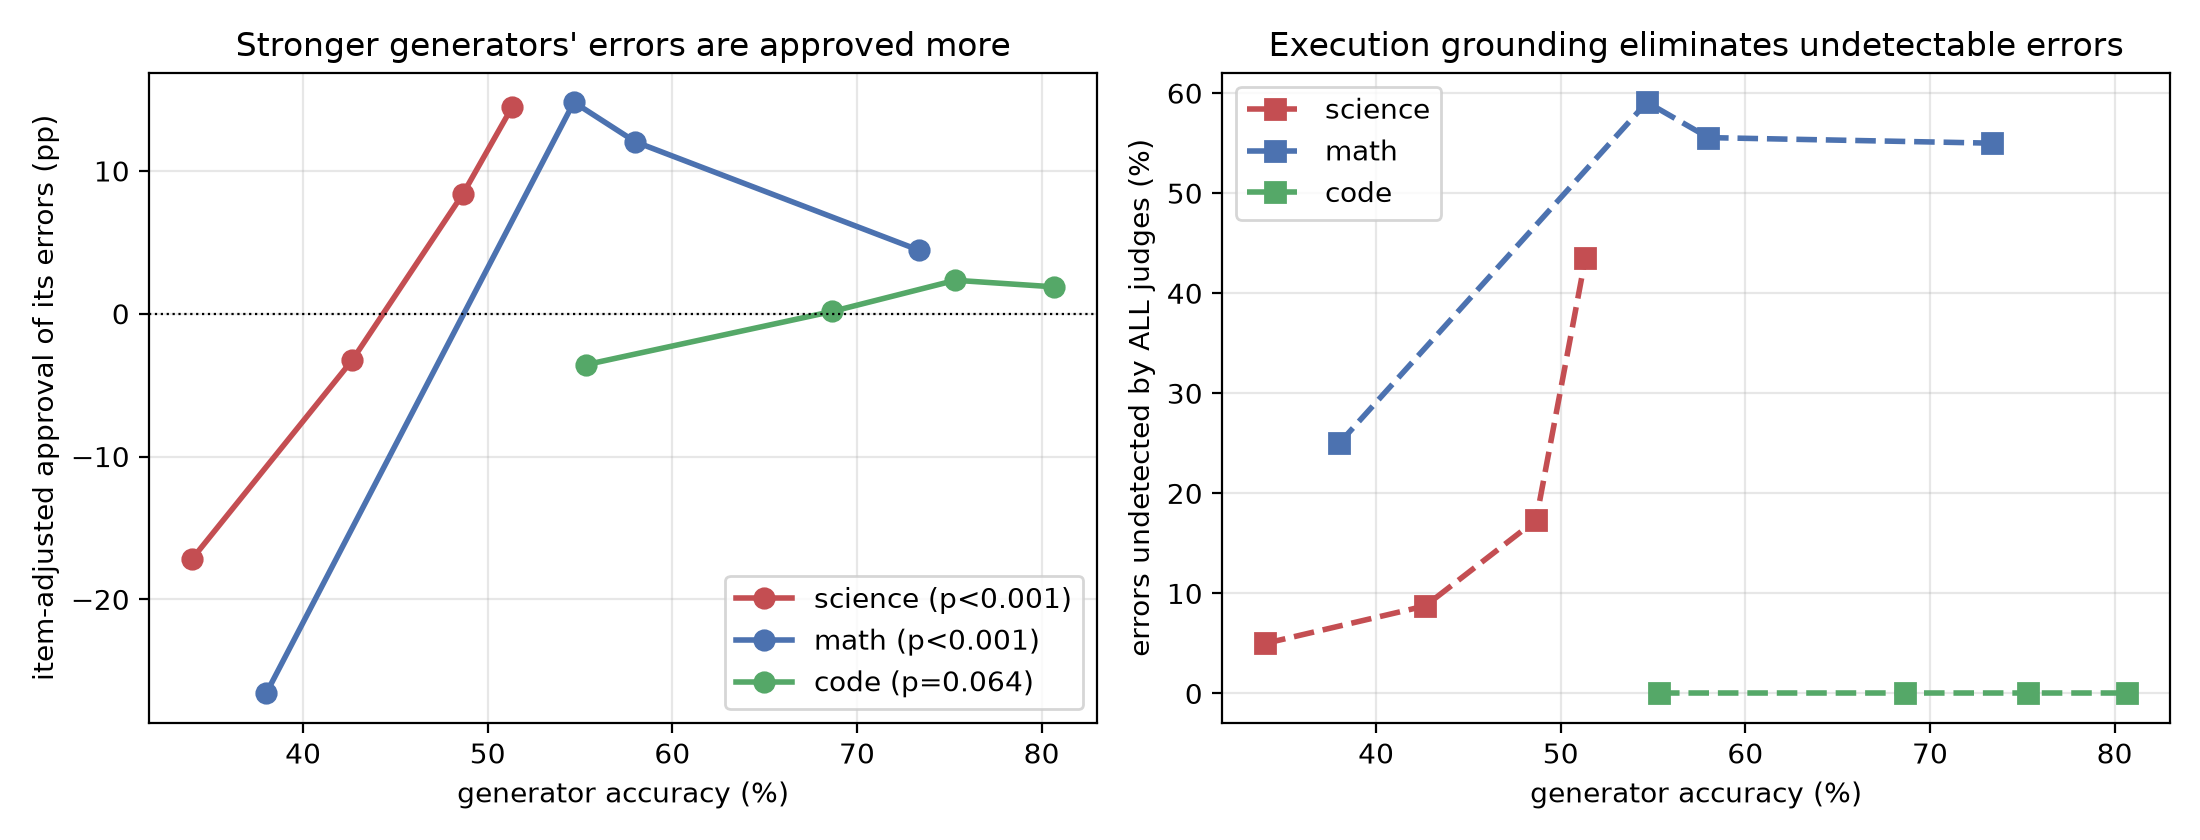
\includegraphics[width=\linewidth]{figures/detectability.png}
  \caption{Item-adjusted approval of a generator's errors vs.\ generator accuracy. Errors from stronger models are significantly harder to catch in math and science ($p < 0.001$), but flat in code ($p = 0.064$).}
  \label{fig:detectability}
\end{minipage}\hfill
\begin{minipage}{0.48\textwidth}
  \centering
  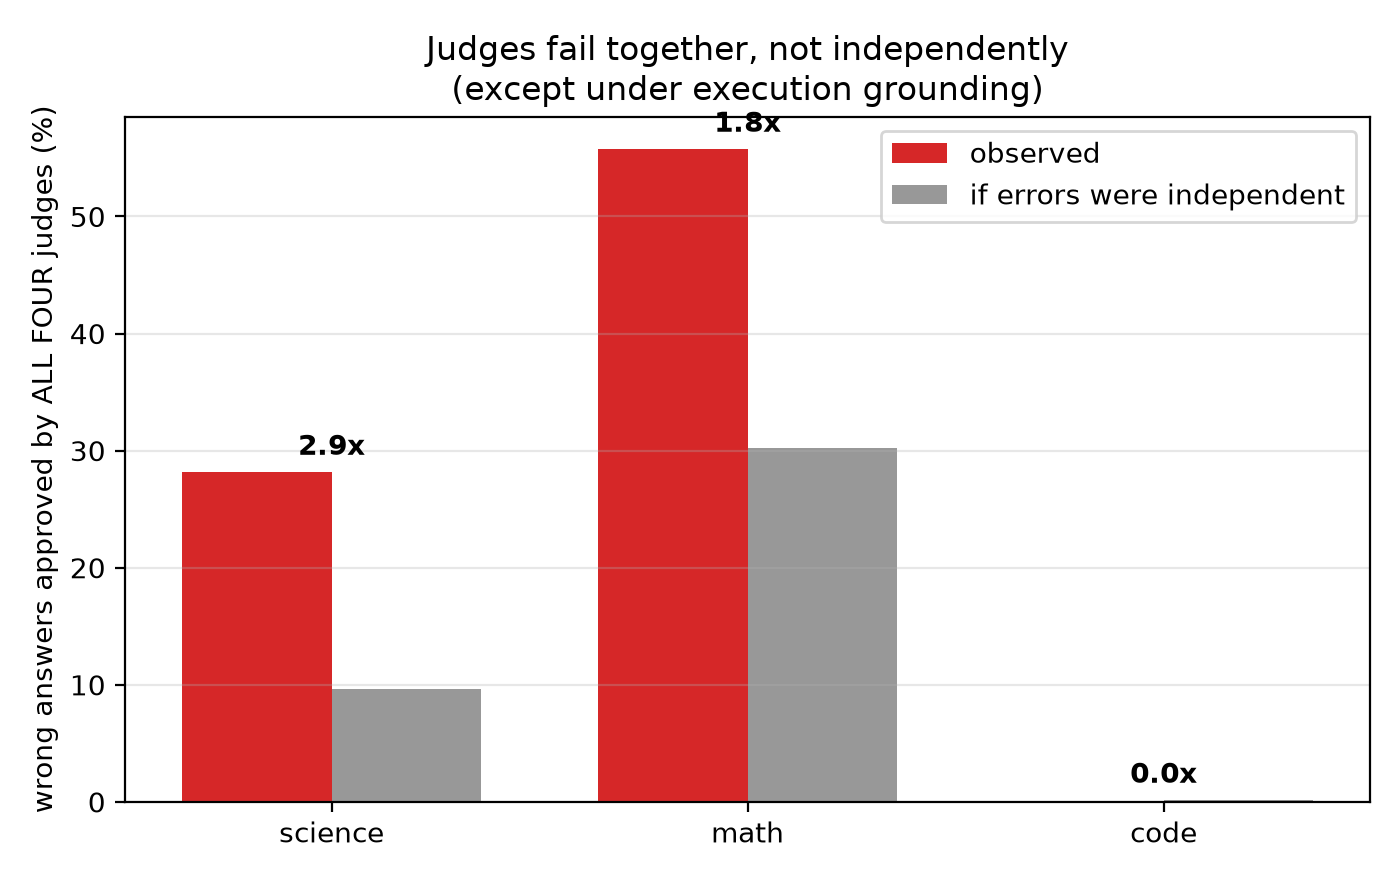
\includegraphics[width=\linewidth]{figures/4_correlated_failure.png}
  \caption{Wrong answers approved by all four judges simultaneously in the full composition pool: observed vs.\ expected under independence. Ungrounded judges share correlated blind spots ($1.8\times\text{--}2.9\times$ chance; $1.5\times\text{--}1.8\times$ in leave-one-out 3-judge panels).}
  \label{fig:correlated-failure}
\end{minipage}
\end{figure}

\paragraph{Detectability Falls with Generator Capability.}
As shown in Figure~\ref{fig:detectability}, in ungrounded domains (science and math), errors produced by more capable generators are systematically harder for any judge to catch. Item-adjusted approval of errors rises sharply with generator accuracy in science ($-17.7$\,pp to $+14.0$\,pp, $p < 0.001$) and math ($-27.0$\,pp to $+14.7$\,pp, $p < 0.001$). In code, however, where execution feedback is present, error detectability remains flat ($-3.7$\,pp to $+2.3$\,pp, $p = 0.064$).

\paragraph{Correlated Failures Neutralize Ensembles.}
The reason voting panels fail in ungrounded domains is that judges do not fail independently. As shown in Figure~\ref{fig:correlated-failure}, pairwise Cohen's $\kappa$ is moderate in ungrounded domains ($\kappa = +0.35$ in science, $+0.45$ in math), where wrong answers deceive all four judges simultaneously $1.8\times\text{--}2.9\times$ more often than expected by chance in the full pool ($1.8\times$ in math, $2.9\times$ in science; $1.5\times$ and $1.8\times$ respectively in leave-one-out 3-judge panels). In code, execution grounding decorrelates errors ($\kappa = +0.09$). Consequently, sweeping all majority-vote thresholds ($k$-of-$N$) reveals that no ensemble beats the best single judge in math or science: panels inherit shared blind spots rather than averaging them away.

\paragraph{The Scale and Override Problem.}
Scaling model size fails to break specificity collapse: leading 70B+ judges achieve an average error catch rate of only $48.9\%\text{--}50.2\%$ across ungrounded tasks. Cross-capability oversight yields diminishing returns: while larger models outperform the 12B model on identical errors (53.1--61.8\% win rates in Table~\ref{tab:oversight-full}), comparisons among the largest models (DeepSeek-671B vs.\ Qwen-72B vs.\ Llama-70B) collapse to near chance (49.7--53.7\%). More critically, in code, leading judges frequently overrule passing test suites: of 1,458 overrides, our differential fuzzing audit found that 77.2\% (1,125 cases) were unconfirmed defects under automated testing, and only 7.3\% (107 cases) caught genuine bugs. Scaling capability increases assertiveness, not ground-truth fidelity.

% =========================================================================
% 4.4 PROPOSED FIX 2: MULTI-AGENT DELIBERATION
% =========================================================================
\subsection{Testing Proposed Fix 2: Multi-Agent Deliberation Juries}
\label{sec:results-jury}

We benchmark two ungrounded multi-agent jury architectures: \textbf{(1) Team A (Parallel Debate):} an unconstrained multi-turn debate between three models (Step 3.7 Flash, Nemotron-4-340B, Kimi K2.7 Code) with an impartial arbiter; and \textbf{(2) Team B (Sequential Pipeline):} a 3-stage role-specialized chain (provable correctness analysis $\to$ boundary-case attack $\to$ instruction-fidelity arbitration).

\begin{table}[t]
\centering
\small
\caption{Deliberation juries (zero grounding) vs.\ execution-grounded verifier on DeepSeek code ($n = 150$). Juries inflate compute ($8\times\text{--}32\times$ tokens, $28\times\text{--}457\times$ cost) but trail grounding by $17\text{--}23$\,pp in error catch rate (TNR).}
\label{tab:jury-comparison}
\begin{tabular}{lccccc}
\toprule
\bf Architecture & \bf Grounding & \bf Balanced Acc & \bf Catch Rate (TNR) & \bf FPR & \bf Cost / Problem \\
\midrule
Team B: Sequential Pipeline  & None & 81.67\% & 70.00\% & 30.00\% & \$0.0056 ($28\times$) \\
Team A: Parallel Debate       & None & 86.67\% & 76.67\% & 23.33\% & \$0.0914 ($450\times$) \\
\midrule
\bf Grounded Baseline: Qwen2.5-72B & \bf Execution & \bf 96.25\% & \bf 93.33\% & \bf 6.67\% & \bf \$\bf 0.0002 ($1\times$) \\
\bottomrule
\end{tabular}
\end{table}

\paragraph{Adversarial Infection in Debate.}
As shown in Table~\ref{tab:jury-comparison}, ungrounded deliberation trails execution grounding ($70.0\%\text{--}76.7\%$ vs.\ \textbf{93.33\%} catch rate). Qualitative analysis reveals the core failure mode: \emph{adversarial infection}. Without execution feedback, when one agent conjectures a pedantic edge case, others concede, falsely rejecting valid code and inflating compute by $28\times\text{--}457\times$ without improving accuracy.

% =========================================================================
% 4.5 SYNTHESIS
% =========================================================================
\subsection{Synthesis: What Actually Fixes an LLM Verifier}
\label{sec:results-synthesis}

\begin{table}[t]
\centering
\small
\caption{Synthesis of verifier interventions. Model-side fixes fail to resolve belief persistence; only execution grounding establishes reliability.}
\label{tab:synthesis}
\resizebox{\linewidth}{!}{%
\begin{tabular}{lp{6.8cm}cc}
\toprule
\bf Intervention Class & \bf Primary Failure Mode Observed & \bf Catch Rate & \bf Cost \\
\midrule
Prompting (Blinding / Rubrics) & Belief persistence ($<1$\,pp shift); unconfirmed code defects ($-10\text{--}37$\,pp) & $43.8\text{--}47.7\%$ & $1.0\text{--}1.2\times$ \\
Scaling \& Oversight & Diminishing returns at scale ($49.7\text{--}53.7\%$); $77.2\%$ unconfirmed test overrides & $48.9\text{--}50.2\%$ & $\sim 5\times$ \\
Panels \& Juries (Debate) & Correlated blind spots ($\kappa \ge 0.35$); debate adversarial infection & $70.0\text{--}76.7\%$ & $3\text{--}457\times$ \\
\midrule
\bf Environmental Grounding & \bf Ground-truth anchor; decorrelates errors ($\kappa = 0.09$); resolves failure & \bf 93.3\% & \bf $1\times$ \\
\bottomrule
\end{tabular}%
}
\end{table}

Our findings demonstrate that: \textbf{blinding fails} because self-preference is rooted in belief persistence, not author labels; \textbf{scaling, ensembling, and debate fail} because ungrounded models share correlated reasoning errors; and \textbf{environmental grounding succeeds} because it decouples verification from generative habits. Verifier reliability is bounded by the ground-truth signals provided by the environment, not the sophistication of the judge.
